\section{Gold-PVD}

Als Testsystem für PVD-Prozesse bietet sich Gold als ein System an, dessen Abscheidungsprozess zwar durch Oberflächendiffusion dominiert wird, jedoch kristalline Strukturen bildet und für das ausgiebig erforschte MD-Parametrisierungen existieren.

\subsection{Voruntersuchungen}

Als kristallines, unäres Abscheidungssystem wurden zur Vorbetrachtung die Bindungslängen, Dichten sowie Koordinationen der kristallinen Phase untersucht\todo{Oberfläche?}.
Eine Stabilitätsanalyse des Precursormoleküles entfällt, da bei PVD-Prozessen nur einzelne Atome auf die Oberfläche aufgebracht werden.
Die Ergebnisse dieser Untersuchungen, die erwartungsgemäß gute Übereinstimmung zwischen Simulation und Experiment zeigen, sind in Tabelle \ref{tab:goldpreresults} zusammengefasst.

\begin{table}[hbtp]
  %% \rowcolors{0}{white}{lightgray} 
  \caption[Eigenschaften von Gold]{Eigenschaften von Gold als Voruntersuchung des PVD-Prozesses. Die Abweichung der Koordinationszahl wird in der Nichtperiodizität der untersuchten Struktur vermutet}
  \label{tab:goldpreresults}
  \begin{tabularx}{\textwidth}{|XXXX|}
    \hline
    \textbf{unters. Größe} & \textbf{Simulation} & \textbf{Experiment} & \textbf{Abweichung}\\
    \hline
    Bindungslänge & 2.879 \AA & 2.884 \AA & 0.2\% \\
    Koordination & 11.81 & 12.00 & 1.6\% \\
    Dichte (300K) & 18.99 g/cm$^3$ & 19.30 g/cm$^3$ & 1.6\%\\
    Dichte (500K) & 18.89 g/cm$^3$ & 19.13 g/cm$^3$ & 1.2\%\\
    \hline
  \end{tabularx}
\end{table}


\subsection{Prozess-Simulation}

Mangels chemischer Reaktionen genügt es, die Auftrefforte der Goldatome zufällig gleichverteilt auf der xy-Ebene auszuwählen.

\subsubsection{Strukturierte Substrate}

Als nächste Stufe wurden strukturierte Substrate untersucht, von denen eine Auswahl in Abbildung \ref{fig:goldsubstrate} dargestellt sind.
Diese wurden per Materials Studio präpariert, per Atomsk in ein kompatibles Format überführt und anschließend von Parsivald eingelesen und mit einzelnen Goldatomen beschichtet.

\begin{figure}[bt]
  \captionsetup[subfigure]{singlelinecheck=false}
  \def\subfigwidth{0.31\textwidth}
  \begin{subfigure}[t]{\subfigwidth}
    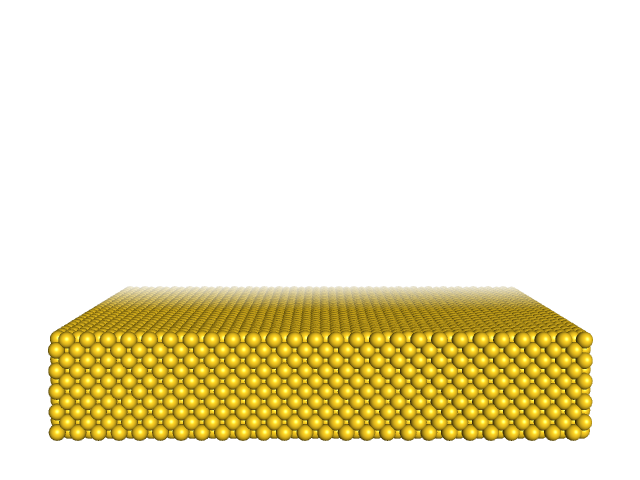
\includegraphics[width=\textwidth]{Au_substrate_flat}
    \subcaption{Flaches Gold-Substrat}
    \label{fig:goldsubstrate-a}
  \end{subfigure}
  \hfill
  \begin{subfigure}[t]{\subfigwidth}
    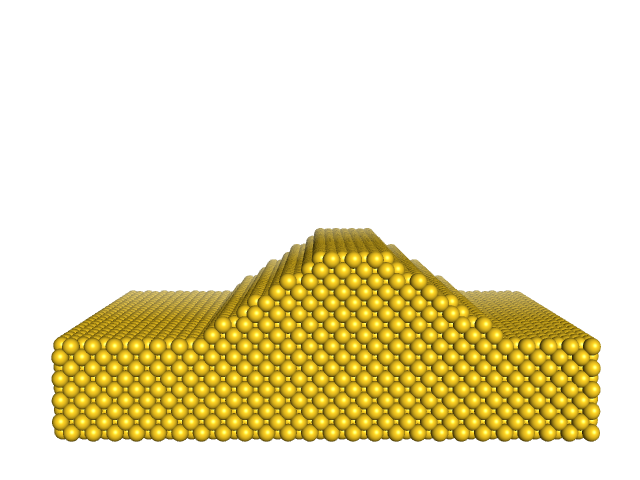
\includegraphics[width=\textwidth]{Au_substrate_step30}
    \subcaption{Gold-Stufe, 30°}
    \label{fig:goldsubstrate-a}
  \end{subfigure}
  \hfill
  \begin{subfigure}[t]{\subfigwidth}
    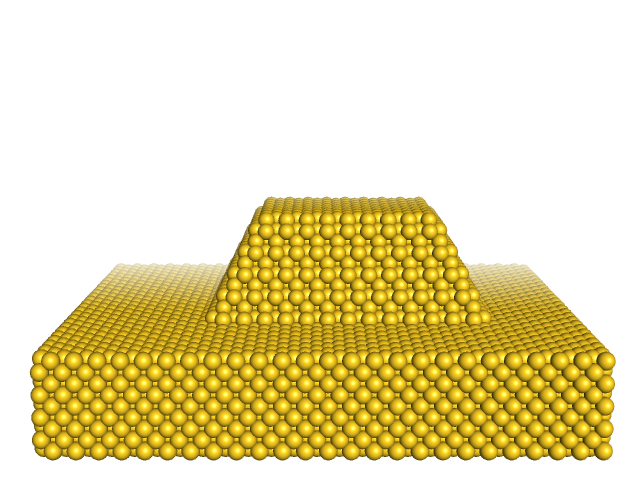
\includegraphics[width=\textwidth]{Au_substrate_tip60}
    \subcaption{Gold-Spitze, 60°}
    \label{fig:goldsubstrate-a}
  \end{subfigure}
  \caption[Strukturierte Goldsubstrate]{Goldsubstrate mit unterschiedlicher Struktur und Breite und Tiefe von 100 \AA.
    Abscheidungen wurden auf flachen Substraten sowie Stufen und Spitzen mit jeweils 15°, 20°, 30°, 45°, 60° und 90° Neigung durchgeführt.}
  \label{fig:goldsubstrate}
\end{figure}

\begin{figure}[bt]
  \captionsetup[subfigure]{singlelinecheck=false}
  \def\subfigwidth{0.31\textwidth}
  \begin{subfigure}[t]{\subfigwidth}
    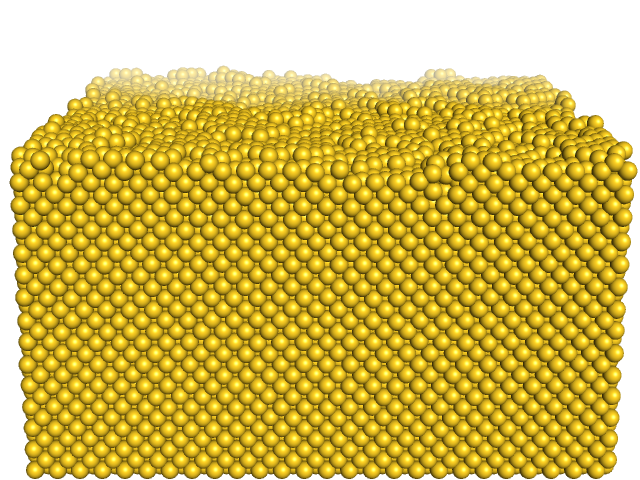
\includegraphics[width=\textwidth]{Au_deposition_flat}
    \subcaption{Abscheidung auf flachem Gold-Substrat}
    \label{fig:goldsubstrate-a}
  \end{subfigure}
  \hfill
  \begin{subfigure}[t]{\subfigwidth}
    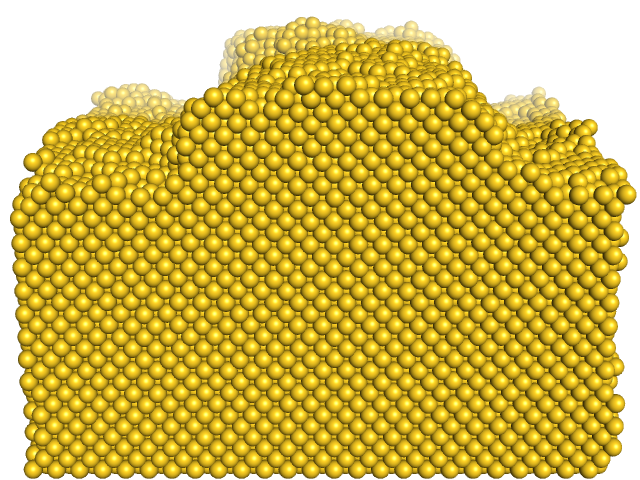
\includegraphics[width=\textwidth]{Au_deposition_step30}
    \subcaption{Abscheidung auf Gold-Stufe, 30°}
    \label{fig:goldsubstrate-a}
  \end{subfigure}
  \hfill
  \begin{subfigure}[t]{\subfigwidth}
    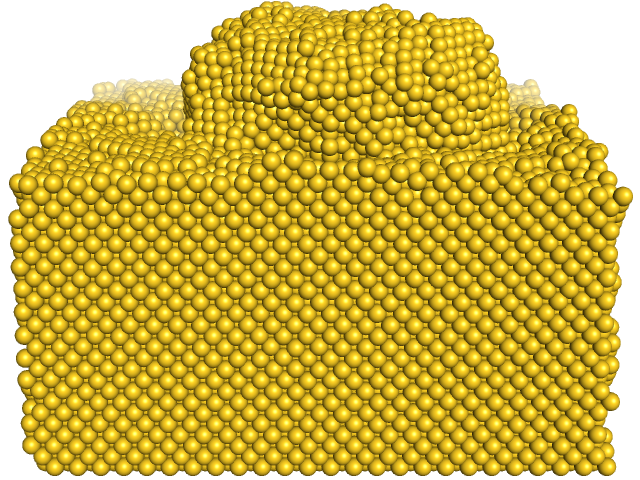
\includegraphics[width=\textwidth]{Au_deposition_tip60}
    \subcaption{Abscheidung auf Gold-Spitze, 60°}
    \label{fig:goldsubstrate-a}
  \end{subfigure}
  \caption[Abscheidung auf strukturierten Substraten]{
    Ergebnis der Abscheidung.
    Die Substratstruktur bleibt erkennbar, wird aber nach oben verstärkt, ansonsten aber kristallin und flach fortgesetzt.
  }
  \label{fig:golddepositions}
\end{figure}

Die Ergebnisse der Gold-Abscheidungen mit Parsivald (Abbildung \ref{fig:golddepositions}) zeigen perfekt fortgesetzte Kristallstrukturen, wobei die Schicht auf dem flachen Substrat nach 10 Kristall-Lagen eine Rauheit von einem Atomdurchmesser zeigt, die weiter beibehalten wird.
Die strukturierten Substrate hingegen zeigen den Trend, die Neigungswinkel an Stufen und Spitzen zu verstärken.
Nach längeren Laufzeiten entstehen somit Überhänge, die durch Abschluss zu Hohlräumen führen, die sich in der Realität durch thermische Relaxation schließen.
Dahinter steht einerseits die Notwendigkeit, Gold-Atome bei Ankunft auf der Oberfläche diffundieren zu lassen, was beim aktuellen Modell nur in Grenzen angewandt wird.

Andererseits steckt dahinter ein methodischer Fehler bei Nutzung von Binning-Methoden:
Die Oberfläche wird aufgrund von Laufzeitbegrenzungen nur entlang der z-Achse bestimmt, woraufhin das neue Atom über einem Atom auf der Oberfläche platziert wird.
Das führt bei Stufen in der Struktur zu Atomen, die immer am oberen Ende einer Kante oder Neigung aufgetragen werden und dort mit statistischer Wahrscheinlichkeit verbleiben.

Eine mögliche Lösung stellt die ausführliche Parametrisierung der Oberfläche dar, beispielsweise per Alpha-Form (Abschnitt \ref{data}, über die man die Ereigniswahrscheinlichkeit entsprechend der Einbettungsenergie, angenähert über die Oberflächenkrümmung, variierte.
